\documentclass[11pt,a4paper]{article}
\usepackage[T1]{fontenc}
\usepackage[utf8]{inputenc}
\usepackage[margin=24mm]{geometry}
\usepackage{lmodern,microtype,amsmath,amssymb,booktabs,array,xcolor,tikz,hyperref}
\usetikzlibrary{arrows.meta,positioning}
\hypersetup{colorlinks=true,linkcolor=teal!60!black,urlcolor=teal!60!black}
\newcommand{\Q}{\mathbb Q}
\newcommand{\Z}{\mathbb Z}
\newcommand{\C}{\mathbb C}
\newcommand{\Tr}{\operatorname{Tr}}
\newcommand{\Ind}{\operatorname{Ind}}
\newcommand{\Reg}{\operatorname{Reg}}
\newcommand{\Urep}{U}
\setlength{\parindent}{0pt}
\setlength{\parskip}{4pt plus 1pt}
\begin{document}
\begin{center}
{\Large\bfseries The six grades of the rank-three table\\[2pt]
and the three winding signs of the Albert frame}\\[4pt]
{\small Research note, 23 November 2026. Arguments developed by OpenAI Codex from the cited September and November work.}
\end{center}

\section*{1. Which phases preserve every product?}
Claude Fable's November calculation gives 132 nonzero coefficients in a ten-element multiplication table over
$\Z[D]$, where $q=v^2\ne0$ and $D=q+2+q^{-1}$. Work with its free ten-element specialization, so the distinguished
labels remain formal basis vectors even at a singular fibre. For an abelian group $B$, assign a degree in $B$ to
each label. A nonzero coefficient of $z$ in $xy$ imposes $d(z)=d(x)+d(y)$. Coefficients themselves have degree zero.
The abelian group presented by these equations classifies all such assignments.

\textbf{Theorem 1.} Over $\C$ this universal group is $\Z/6$ at $q=-1$, $\Z$ at the two primitive cube roots,
and zero at every other $q\ne0$. The table gives the universal degrees. The subscript $i$ is the cell number.
\[
\begin{array}{c|rrrrrr}
 & 1 & \Sigma & \gamma^1_1,\gamma^1_2 & \gamma^1_{12},\gamma^1_{21}
             & \gamma^2_1,\gamma^2_2 & \gamma^2_{12},\gamma^2_{21}\\ \hline
D=0\quad(\bmod\,6)&0&3&1&2&3&0\\
D=1\quad(\Z)&0&2&1&1&1&1
\end{array}
\]
\textit{Proof.} Write $S=\Sigma$. Its square is $4D^2(D-1)^2 S$.
Multiplication of $S$ by $\gamma^i_w$ gives $D^{|w|-1}G_i S$ with
$G_1=4D(D-1)$ and $G_2=D^2(D-1)$. Away from $D=0,1$ these relations force all ten degrees to be zero.
At $D=1$ every one of the 64 ordered products of two $\gamma$'s equals $S$, and $S$ annihilates the nine nonunit
labels. Holding one factor fixed identifies all eight $\gamma$ degrees. Their common degree $x$ is free and $d(S)=2x$.

At $D=0$, suppress nonzero numerical coefficients. In cell one write $a,b$ for the one-letter labels and $u,v$ for
the two-letter labels. The products $ab=u$, $ba=v$, and the terms $av,ua,bu,vb$ supported on $S$ give
$d(u)=d(v)=d(a)+d(b)$ and $d(S)=2d(a)+d(b)=d(a)+2d(b)$. Thus $d(a)=d(b)=x$ and $d(S)=3x$.
Use capitals $A,B,U',V'$ for cell two. The squares of $U',V'$ are supported on themselves, so both have degree
zero. The supports of $AB,BA$ give $d(A)+d(B)=0$. The product $AV'$ has both $S$ and $A$ in its support, and
$BU'$ has both $S$ and $B$. Thus $d(A)=d(B)=d(S)$ and $6x=0$.
Conversely the displayed degrees satisfy every surviving relation. Besides the 19 unit coefficients,
the first cell has the six terms just listed. The second has $AB,BA$, the two squares, and $AV',U'A,BU',V'B$,
each of these last four having two terms. There are no cross-cell terms. Hence order six is attained.
The last equivalence uses $D=(q+1)^2/q$ and $D-1=(q^2+q+1)/q$. \hfill$\square$

Pair this grading at $q=-1$ with the sign character $d\mapsto(-1)^d$. It gives five even and five odd basis
vectors. Its trace is zero on a ten-dimensional algebra. Pair it with $d\mapsto\omega^d$, $\omega^3=1$,
$\omega\ne1$. Its trace is $6+2\omega+2\omega^2=4$. These are diagonal algebra automorphisms. The cyclic trace
identity on the corrected $2\times2$ matrix block, established earlier in NEG\_NIGHT NN-G012, cyclically permutes
three arguments of a trilinear form. The two calculations therefore have different conclusions.

\newpage
\section*{2. Where the two 24-dimensional actions agree}
The September Jordan proof turns an eigenframe by half the angle of its matrix loop. One full turn gives
$D_{12}=\operatorname{diag}(-1,-1,1)$. Conjugation fixes the three scalar diagonal entries and changes sign on
two octonion blocks. The three returns form $V_4$. The cyclic frame permutation rotates its three nonidentity
elements. Together they generate $A_4=V_4\rtimes C_3$. Separately, the marked Golay construction in the September
Leech proof gives an $A_4$ acting by permutations on 24 coordinates, with the three octad traces rotated by $C_3$.

Let $U$ be the regular representation of $A_4/V_4$ inflated to $A_4$. Let $T$ be the tetrahedron's permutation
representation on four vertices with its invariant line removed. Its character on the identity, a double
transposition and a three-cycle is $(3,-1,0)$. The values agree on the two classes of three-cycles.
For every nontrivial sign $\ell$ of $V_4$, $T=\Ind_{V_4}^{A_4}\ell$, as is seen by restricting the three conjugate
signs to $V_4$ and taking the trace on its other cosets.

\textbf{Theorem 2.} The two September actions have the following rational characters. Write $K=\ker(P)$ for the
kernel of the three integral Leech traces.
\[
\begin{array}{l|c|rrr}
 & \text{decomposition}& 1 & (12)(34) & (123)\\ \hline
\text{Albert diagonal} & U          &3&3&0\\
\text{Albert off-diagonal} & 8T     &24&-8&0\\
\text{full Albert space }J & U+8T   &27&-5&0\\
\text{Leech coordinate space }\Lambda_{\Q} & 2U+6T &24&0&0\\
\text{Leech trace kernel }K_{\Q} & U+6T&21&-3&0
\end{array}
\]
\textit{Proof.} The stabilizer of a marked octonion block is $V_4$ and acts there by one scalar sign.
Inducing its eight copies gives $8T$. On the Golay side the six $V_4$-orbits on coordinates each have size four.
All elements outside $V_4$ rotate the three octads. Thus every nonidentity element acts without fixed coordinates.
The 24 coordinates give two regular $A_4$-orbits. Each regular representation is $U+3T$.
The surjection $P$ has quotient $U$. Semisimplicity in characteristic zero gives the last row.
\hfill$\square$

\begin{center}
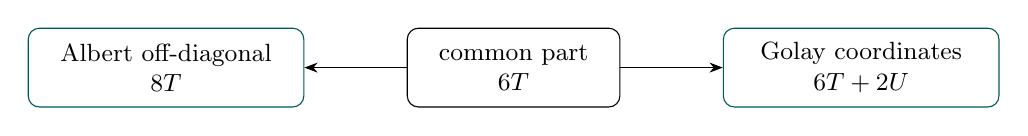
\begin{tikzpicture}[>=Stealth,node distance=6mm,font=\small]
\node[draw=teal!70!black,rounded corners,align=center,minimum width=35mm,minimum height=10mm] (a)
 {Albert off-diagonal\\$8T$};
\node[draw,rounded corners,align=center,right=13mm of a,minimum width=27mm,minimum height=10mm] (b)
 {common part\\$6T$};
\node[draw=teal!70!black,rounded corners,align=center,right=13mm of b,minimum width=35mm,minimum height=10mm] (c)
 {Golay coordinates\\$6T+2U$};
\draw[->] (b) -- (a); \draw[->] (b) -- (c);
\end{tikzpicture}\\[-1pt]
{\small Arrows denote possible rational inclusions. A particular inclusion requires a choice.}
\end{center}
Both 24-dimensional representations restrict to eight regular triples on $C_3$. Their largest common $A_4$
subrepresentation has dimension 18. A sign winding separates them, since their traces there are $-8$ and zero.
On the full Albert space the eigenvalues at a winding of order two have multiplicities $(11,16)$.
A three-cycle has nine copies each of $1,\omega,\omega^2$. Its first and second traces vanish and its third is 27.

\textbf{Integral consequence.} September's trace theorem proves $P(\Lambda)=\Z^3$, $P(\Lambda^{V_4})=4\Z^3$.
For any integer lift $b$ of $t$, the cocycle $h\mapsto hb-b$ defines an element of $H^1(V_4,K)$.
It vanishes precisely when $t$ has an invariant lift, and is additive in $t$. Its image is therefore
$(\Z/4)^3$, with $C_3$ rotating coordinates. Over $\Z/4$, the projector $(1+C+C^2)/3$ splits the diagonal
from the sum-zero plane. The cyclic differences $v=(1,-1,0)$ and $Cv$ form a basis for that plane, with
$(1+C+C^2)v=0$. Its module is $\Z[\omega]/4$, and its reduction modulo 2 is $\mathbb F_4$.
This locates the order-four obstruction in one invariant direction and one pair of rotating differences.

\newpage
\section*{3. Which extended RH assertion the frame detects}
Give the finite actions in Theorem 2 an arithmetic realization by specifying a Galois extension $N/\Q$ with
group $A_4$. Write $C=N^{V_4}$ and $F=N^{C_3}$ for the cyclic cubic and quartic subfields. Put $L_T=L(s,T)$.
The two traces now determine exactly which global $L$-function has to be understood. This construction uses the
chosen Galois quotient. The September real frame by itself supplies no choice of $N$.

\textbf{Theorem 3.} Including the ramified finite factors, one has
\[
\begin{aligned}
 L_T&=L_C(s,\ell)=\zeta_F(s)/\zeta(s),&
 \zeta_N&=\zeta_C L_T^3,\\
 L(s,J)&=\zeta_C L_T^8,&
 L(s,\Lambda_{\Q})&=\zeta_C^2 L_T^6,\qquad L(s,K_{\Q})=\zeta_C L_T^6.
\end{aligned}
\]
For this $N$, RH for $\zeta_F$, RH for $\zeta_N$, RH for $L(s,J)$, and simultaneous RH for all
$A_4$-representations are four equivalent assertions. Each is equivalent to RH for the single quadratic
Hecke character $\ell$ over $C$. Its three conjugates have the same induced $L$-function. For an individual
representation the same equivalence holds whenever $T$ occurs.

\textit{Proof.} The action on tetrahedron vertices is $1+T=\Ind_{C_3}^{A_4}1$. The action on the three cosets
of $V_4$ is $U$. Direct sum multiplies Artin factors and induction gives the $L$-function over the fixed field.
Use these identities on the decompositions in Theorem 2 and on $\Reg(A_4)=U+3T$. Artin formalism takes inertia
invariants at ramified primes. By abelian class field theory $L_C(s,\ell)$ is a nontrivial finite-order Hecke
$L$-function and is entire. The other three complex irreducibles are the characters of the cyclic cubic
quotient. Their $L$-functions are rational Dirichlet factors already covered by Alpöge's theorem.
In the open critical strip all these factors are holomorphic. In any representation containing $T$ an off-line
zero of $L_T$ therefore persists with positive multiplicity. Conversely these four irreducibles exhaust the group.
This also proves the assertion for all tensor and Schur functors on the frame. \hfill$\square$

\textbf{What remains for this choice of frame.} At the level of $A_4$ there is a single remaining analytic
factor after Dirichlet GRH. The older $S_3$ example in the conversation induces an order-three character
over $\Q(\omega)$, producing a degree-two function over $\Q$. The tetrahedral example instead cycles three
order-two characters and produces a degree-three function. The finite degrees are compatible with global
Artin induction in both cases. It is the arithmetic distribution of the characters at primes that remains.

\newpage
\section*{3.1. Computing the three signs at a rational prime}
Take $N$ to be the splitting field of $f(X)=X^4+8X+12$.
Its discriminant is $576^2$. The three pair-partition resolvent has polynomial
$Y^3-48Y-64$, which after $Y=4Z$ is $64(Z^3-3Z-1)$. The cubic has no rational root.
The quartic has no linear factor since its real minimum is $12-6\sqrt[3]2>0$. A rational splitting into two
quadratics would fix a pair partition and give a rational resolvent root. Thus the quartic is irreducible.
Its Galois group is transitive, lies in $A_4$, and acts transitively on the pair partitions. Its order is divisible
by both four and three, so it is $A_4$. Here $C=\Q(2\cos(\pi/9))$ is the real cyclotomic cubic of conductor nine.

Write $z=2\cos(\pi/9)$. The sign $\ell$ can be taken to be the quadratic character of $C(\sqrt z)/C$.
Indeed for roots $r_i$ of $f$, the three squared pair sums $(r_1+r_i)^2$, $i=2,3,4$, are its three resolvent
roots. To see this, use $\sum r_i=\sum_{i<j}r_ir_j=0$ to write
$(r_1+r_2)^2=r_1r_2+r_3r_4$ and permute. The resolvent roots are $4z_i$, with $z_i$ the conjugates of $z$.
The subgroup $V_4$ fixes each pair partition. On a chosen sum it acts through a nontrivial sign since one
double transposition exchanges the pair and its complement. The other sums give the conjugate signs.
Their squares have product $4^3$, and $N_{C/\Q}(z)=1$.

At $p>3$ the exact unramified trace is therefore the directly computable integer
\[
 t(p)=\#\{x\bmod p:f(x)=0\}-1
     =\sum_{\substack{a\bmod p\\ a^3-3a-1=0}}\left(\frac ap\right).
\]
If $p\not\equiv\pm1\bmod9$ the cubic is inert, the sum is empty, and a three-cycle has trace zero.
Otherwise the three roots give three residue symbols of product one. All positive gives trace 3, and precisely
two negative gives trace $-1$. These are exactly the two possibilities inside $V_4$. This also proves the
formula by induction of the character, without a numerical assumption about splitting.

\textbf{Conductor and real places.} The unit $z$ is negative at exactly two of the three real embeddings.
All odd finite places are unramified in $C(\sqrt z)/C$. The prime 2 is inert in $C$. The polynomial
$Z^3-3Z-1$ has odd discriminant and its reduction gives $\mathbb F_8$. In that residue field the unique square
root of $z$ is $z^4$. In the integer ring $z^8-z=28z^2+26z+6\equiv2(z+1)\pmod4$, which is nonzero modulo 4.
Every lift of $z^4\bmod2$ has the same square modulo 4. Thus $z$ is no square modulo 4. Locally the order
generated by $\sqrt z$ has discriminant $4z$. An index-two-ideal enlargement would contain
$(a+\sqrt z)/2$ after rescaling by a unit, whose norm forces $a^2\equiv z\bmod4$. To justify that form, any
new integral element in half the order has such a numerator with unit coefficient of $\sqrt z$: a nonintegral
element of the base field cannot become integral in the extension. An enlargement by more than one uniformizer
in the index is impossible by the discriminant valuation two. Hence the relative discriminant and conductor are
$(4)$. The two nontrivial characters of $C/\Q$ both have conductor 9, so $|D_C|=81$. The conductor of $T$ is
$81\,N_{C/\Q}(4)=5184$. Its three real factors are $\Gamma_{\mathbb R}(s)\Gamma_{\mathbb R}(s+1)^2$.

At $p=5$, $f$ factors into a linear and an irreducible cubic polynomial. Frobenius is a three-cycle.
With $u=5^{-s}$ its Albert Euler denominator is $(1-u^3)^9$. The linear coefficient is zero, yet this factor
contains all 27 local degrees. At a double transposition the denominator is
$(1-u)^{11}(1+u)^{16}$. These formulas follow directly from Theorem 2 and give a way to read the cancellation
in the split-zero construction prime by prime.

\newpage
\section*{4. How to insert a winding into the sign calculation}
The finite-field proof in the H01 manuscript identifies the signed remainder with the Frobenius trace of the
actual space $W=V^{\otimes k}\oplus K_k$, where $K_k$ is the kernel of a surjective Gysin map. This is the
point at which all spectral multiplicities acquire the same sign. Suppose an $A_4$-action preserves the sheaf,
cut and maps in that exact sequence and commutes with Frobenius $F$. The projector onto the three nontrivial
$V_4$-characters is
\[
 P=1-\tfrac14\sum_{h\in V_4}h,\qquad
 \Tr(F^n\mid PW)=\tfrac34\Tr(F^n\mid W)
                  -\tfrac14\sum_{1\ne h\in V_4}\Tr(hF^n\mid W).
\]
Indeed the average projects onto invariants. Applying $P$ to the exact Gysin sequence preserves exactness and
leaves an actual kernel. On the Albert frame the right side at $F=1$ is $(3\cdot27-3(-5))/4=24$. On the
Leech space it is 18. Thus the three winding traces extract the respective off-trivial sign sectors exactly.
A geometric application to H01 requires an action preserving the chosen cut and estimates for its twisted
trace sums. In the number-field proof the analytic input is a one-sided prime-window estimate. This finite
projection identifies an effective space but supplies no such bound.

There is also an exact rule when $F$ \emph{permutes} three marked eigenspaces
$W_0\to W_1\to W_2\to W_0$ isomorphically. Put $B=F^3|_{W_0}$. Using $F$ to identify the other slots with
$W_0$ makes $F$ a block cycle with return map $B$. Consequently
\[
 \det(1-uF)=\det(1-u^3B),\qquad
 \Tr(F^n)=
 \begin{cases}0&3\nmid n,\\3\Tr(B^{n/3})&3\mid n.\end{cases}
\]
The first two zero traces retain the entire returning space. This calculation uses genuine powers of one
operator. A single reflection inserted afresh into each trace can erase a rotating space at every power.

\textbf{The distinction in Alpöge's own argument.} In the number-field proof the Mellin transform of a window
has residue $m_\rho/(\rho(1-\rho))$ at a real zero $0<\rho<1$ of multiplicity $m_\rho$.
It is positive. For an admissible character family the formal deduction
\texttt{zeroFree\_of\_rpow\_window} uses an \emph{upper} bound $G(y)\le C y^\theta$ on arbitrarily late
intervals $[Y,Y^{1+\delta}]$, with $\delta>0$ and $0<\theta<1$. It returns zero-freeness to the right of
$\theta$. The arithmetic work is to produce these windows. Phases already enter the metaplectic construction
in Alpöge's remark, while the residue sign appears after taking the logarithmic derivative.
In particular a positive trace multiplicity for the finite $A_4$ representation in Theorem 3 supplies the
representation to which one wants to apply an arithmetic estimate. The estimate is a separate assertion.

\newpage
\section*{5. Mirroring the three colours and retaining the sign}
The November discussion asked what happens to the original signed pairing on doubling a three-way space.
Let $R$ be a unitary rotation with $R^3=1$ on $E$, and let $J$ be a unitary involution with $JRJ=R^{-1}$.
On $E\oplus E$ write $S$ for exchange of sheets. There are two rotations
\[
 R_+=\operatorname{diag}(R,R),\qquad R_-=\operatorname{diag}(R,R^{-1}).
\]
The normalized graph map $i(x)=(x,Jx)/\sqrt2$ is an isometry and satisfies
\[
 iJ=Si,\quad iR=R_-i,\quad \langle ix,Six\rangle=\langle x,Jx\rangle.
\]
Thus it is an explicit lift of the original form. Exchange commutes with $R_+$ and inverts $R_-$.
What can a different linear lift retain if its new rotation commutes with its new sign?

\textbf{Proposition.} Every linear intertwiner $L$ from $(E,R,J)$ to a commuting rotation $R'$ and
involution $J'$ annihilates both nontrivial $C_3$ eigenspaces (over $\C$). Indeed
$LR^{-1}=LJRJ=J'R'J'L=R'L=LR$. The operator $R-R^{-1}$ is invertible on the $\omega$ and $\omega^2$
eigenspaces. Conversely the quotient by those two spaces has trivial rotation, and the sign descends.
Consequently the largest quotient that such a lift can retain is the rotation-invariant part. This proves
the precise information loss in commuting the marked complement with the marked rotation. The doubled
space still realizes both actions. A correspondence with an additional kernel could carry more information.

\textbf{A finite arithmetic example from September.} Return to the arithmetic notation in which $p$ is prime,
$p\equiv1\bmod24$, $p/4<a<p/2$, $R=4a-p$ and $S=pa$. Assume $R>1$, so $(R,S)=1$. For real $\sigma$, put
$w(r)=\sum_{d\mid S,\ d\equiv r\bmod R}(d/\sqrt S)^{-\sigma}$ on $G=(\Z/R)^\times$ and
$A(g)=\sum_{r\in G}w(r)w(gr)$. Then $A(-1)>0$ detects an occupied opposition shell.
If $c\in G$ has order three, set $P_0w(r)=(w(r)+w(cr)+w(c^2r))/3$. Orthogonality of characters, or
expansion on each three-element orbit, gives
\[
 A(c)=A(c^2)=\frac{3\lVert P_0w\rVert^2-\lVert w\rVert^2}{2}.
\]
An orbit with entries $x,y,z$ contributes $xy+yz+zx$. Hence $A(c)>0$ exactly when two \emph{distinct}
residues in some $c$-orbit carry divisors. Take the September manuscript's empty shell (7.5),
$(p,a)=(73,25)$. The six divisors of $1825$ give residues $1,5,25,19,14,16$ modulo 27.
For $c=10$ the three occupied orbits are $\{1,10,19\},\{5,23,14\},\{25,7,16\}$, each with exactly two
occupied entries. Hence $A(1)=6$, $A(10)=A(19)=3$ and $A(-1)=0$ at $\sigma=0$. This recovers the empty
opposition shell and evaluates the cubic readout there. Moreover $10^3=1$ modulo 27 whereas
$10^2+10+1\equiv3$ modulo 27. When counting a fixed phase by a norm congruence over residue rings, cancellation
of the factor $c-1$ requires a unit.

{\footnotesize
\textit{Proof sources.} The September 11 notes \emph{Three-coordinate Jordan arithmetic} (coherent returns)
and \emph{Integral inverse maps from Leech trace data} (all triples lift, exact invariant-lift obstruction);
September 12 \emph{Octad-aligned octonions} (two failed descents).
The November 21 exchange, messages 16664, 16795, 16965, 17109, 18003 and 19062, and Claude Fable's
\emph{Counting construction}, Theorems 1--2 and the original 132 coefficients.
For the arithmetic input see \href{https://math.mit.edu/~drew/grh/}{Sutherland's formal checks},
\href{https://www.jmilne.org/math/CourseNotes/CFT.pdf}{Milne, Class Field Theory, Artin $L$-series},
and \href{https://alpo.ge/remark.pdf}{Alpöge's description}. For the finite-field input see the local H01
\emph{deligne\_sign\_only\_v5}, proposition on the signed remainder. The accompanying collection gives the
individual proof and transcript locations.}
\end{document}
